\documentclass[11pt]{book}
\usepackage{amssymb,graphicx,amsmath,mathtools,float,subfig}
\usepackage{lscape}
\usepackage{listings}
\usepackage[utf8]{inputenc}
\usepackage[spanish, es-tabla]{babel}




\usepackage[Bjornstrup]{fncychap}

\usepackage{fancyhdr}
\pagestyle{fancy}
\fancyhf{}
\renewcommand{\headrulewidth}{0.5pt}
\fancyfoot[LE,RO]{\thepage}
\fancyhead[RO]{\slshape\nouppercase{\rightmark}}
\fancyhead[LE]{\slshape{\leftmark}}


\usepackage{indentfirst}	% Tabular tras un section
\usepackage[linktocpage]{hyperref}
\hypersetup{
	colorlinks=false,
	citecolor=black,
	filecolor=black,
	linkcolor=red,
	urlcolor=black,
	pdfborderstyle={/S/U/W 1}
}

\usepackage[svgnames]{xcolor}
\definecolor{griscaption}{RGB}{100,100,100}
\usepackage{caption}
\usepackage[font={color=griscaption},figurename=Fig.,labelfont={bf}]{caption}


\newtheorem{theorem}{Teorema}
\newtheorem{corollary}[theorem]{Corolario}
\newtheorem{lemma}[theorem]{Lema}
\newtheorem{proposition}[theorem]{Proposición}
\newtheorem{definition}[theorem]{Definición}


% Fracciones más grandes
\newcommand\ddfrac[2]{\frac{\displaystyle #1}{\displaystyle #2}}

% Línea vertical para separar imágenes
\newcommand{\rulesep}{\unskip\ \vrule\ }

% Para solucionar el problema de títulos de secciones muy largos
\newcommand{\markedsection}[2]{\section[#2]{#2%
\sectionmark{#1}}
\sectionmark{#1}}

\newcommand{\markedchapter}[2]{\chapter[#2]{#2%
\chaptermark{#1}}
\chaptermark{#1}}

\definecolor{background}{rgb}{1.0, 0.96, 0.96}
\definecolor{emphasis}{rgb}{0.2,0.0,0.0}

\definecolor{gray97}{gray}{.97}
\definecolor{gray75}{gray}{.75}
\definecolor{gray45}{gray}{.45}
\definecolor{gray30}{gray}{.97}

\lstset{
	frame=Ltb,
	framerule=0.5pt,
	aboveskip=0.5cm,
	framextopmargin=3pt,
	framexbottommargin=3pt,
	framexleftmargin=0.1cm,
	framesep=0pt,
	rulesep=.4pt,
	rulesepcolor=\color{black},
	%
	stringstyle=\ttfamily,
	showstringspaces = false,
	basicstyle=\scriptsize\ttfamily,
	commentstyle=\color{gray45},
	keywordstyle={\color{emphasis}\bfseries},
	%
	numbers=left,
	numbersep=6pt,
	numberstyle=\tiny,
	numberfirstline = false,
	breaklines=true,
	literate={Ó}{{\'O}}1{í}{{\'i}}1{ó}{{\'o}}1,
	escapeinside={(*}{*)}
}

 
 
% minimizar fragmentado de listados
\lstnewenvironment{listing}[1][]{\lstset{#1}\pagebreak[0]}{
	\pagebreak[0]
}

\lstdefinestyle{PythonCode}{
	basicstyle=\small,
	frame=single,
	backgroundcolor=\color{background},
	language=Python,
	numbers=left,
	emph={%  
		Para, cada, en, Desde, hasta, Si, Sino, Devuelve %
	},emphstyle={\color{emphasis}\bfseries}
}

 
\lstdefinestyle{Console}{
	basicstyle=\scriptsize\bf\ttfamily,
	backgroundcolor=\color{gray30},
	frame=single,
	numbers=none
}





\begin{document}
\markedchapter{Implementación}{Implementación de un software para la aproximación de órbitas}
\label{chap:implementation}
Una vez hemos estudiado el método de Laplace para la determinación de órbitas mediante tres observaciones, nos centraremos en desarrollar un programa que sea capaz de realizar estos cálculos y mostrar los resultados de manera visual para hacer más fácil la aproximación. Además, éste nos servirá de ayuda para comprobar la precisión con la que se determina una órbita mediante el método laplaciano.\\

Antes de hablar sobre el programa y todas sus funcionalidades, centrémonos en las herramientas que se han utilizado para todo el desarrollo.\\

\section{Herramientas utilizadas.}
\label{sec:herramientas}
Tal y como comentamos en la introducción, todo el código implementado para el funcionamiento de nuestro software está en lenguaje Python. Uno de los motivos por los que se ha tomado la decisión de elegir este lenguaje de programación es el hecho de que durante la carrera nos hemos familiarizado con él dado que en muchas asignaturas hemos requerido su uso. En primer momento se pensó en utilizar C++ por su velocidad y optimización, además de que también se ha utilizado durante la carrera, pero dado que solo necesitábamos hacer unos cálculos sin ninguna carga computacional alta, se decidió tomar Python.\\

Aún así hay un motivo más importante por el que se ha elegido Python, concretamente dos, llamados \textit{Numpy} \cite{numpy} y \textit{Matplotlib} \cite{matplotlib}. Mediante estas dos bibliotecas matemáticas el desarrollo del método de determinación y la posterior visualización de resultados se hace mucho más fácil, y su instalación (como la de la mayoría de bibliotecas de Python) es fácil y rápida, por lo que el código podrá ser utilizado fácilmente en diferentes ordenadores.\\

Junto a estas dos librerías, básicas en Python, hemos utilizado también \textit{seaborn} \cite{seaborn} (basada en \textit{Matplotlib}) para mejorar la visualización de datos, \textit{Astropy} \cite{astropy} para ayudarnos con las conversiones de ángulos y fechas, \textit{requests} \cite{requests} para hacer web scraping (método del que hablaremos más adelante) y \textit{scipy} \cite{numpy} y \textit{sympy} \cite{sympy} para ayudarnos con las aproximaciones numéricas.\\

Por otra parte, hemos utilizado el paquete \textit{Tkinter} \cite{tkinter}, el cuál suele venir por defecto en la instalación de Python, para realizar una interfaz y facilitar el uso del software de determinación de órbitas implementado.\\

Dado que no se conocía por completo el funcionamiento de cada una de estas librerías, se ha utilizado la documentación oficial de cada una de ellas (citada junto al nombre del paquete) para el desarrollo del programa informático por completo.\\

Durante el desarrollo de esta memoria, hemos utilizado GIT y la plataforma GitHub para mantener las versiones del proyecto y facilitar el acceso al código a quien lo necesite. Respecto a este documento, está desarrollado por completo en \LaTeX, elegido porque nos proporciona un formato consistente y elegante. Finalmente, el código ha sido desarrollado utilizando el entorno de desarrollo (IDE) Spyder.\\

Una vez comentadas las distintas herramientas con las que hemos implementado nuestro software, pasemos a ver el funcionamiento del núcleo de éste.\\

\section{Núcleo de la aplicación.}
\label{sec:kernel}
A la hora de desarrollar el código que se encargue de la determinación de órbitas, se ha ido separando el código en función de cuál es su cometido en diferentes archivos y carpetas. Así, la aplicación estará dividida en los directorios \texttt{scripts}, que se encargará de la base para la determinación, \texttt{utils} que contendrá código útil para utilizar en diferentes momentos, y \texttt{test} que contendrá archivos con los que comprobar el correcto funcionamiento del programa. Dado que finalmente acabaremos utilizando una interfaz gráfica, no será necesario comentar el contenido del directorio \texttt{test}. Comentemos a continuación las principales funcionalidades de cada uno de estos archivos.\\

\subsection{Elementos orbitales a partir de la posición y velocidad.}
\label{subsec:orbital_elements_code}
Si disponemos de los valores de la posición y velocidad de un cuerpo en un momento determinado, podremos obtener los elementos orbitales de éste tal y como comentamos en \ref{sec:elements_determination}. Por tanto, será lo primero en lo que nos centremos a la hora de implementar el código, y más tarde nos centraremos en el método de Laplace.\\

Para empezar, se ha creado una clase \texttt{OrbitalObject} que contendrá los elementos orbitales $(a,e,i,\Omega,\omega)$ que definen la órbita de un objeto junto a su nombre y su período $p$. En dicha clase se implementarán diferentes funciones para disponer de los ángulos en grados o radianes, así como la sobrecarga del método \texttt{\_\_str\_\_} para mostrar adecuadamente los valores de un objeto de esta clase por pantalla. Una vez creada la clase, definimos distintos objetos que guardaremos en \texttt{utils/my\_constants.py} para un uso futuro, y así de paso comprobamos su correcto funcionamiento.
\begin{lstlisting}[style=PythonCode]
Earth = OrbitalObject(name='Earth',
                      a=9.997843564797363E-01,
                      e=1.707168344231522E-02,
                      i=1.982259124359018E-03,
                      Omega=2.194445465875467E+02,
                      omega=2.426369002793497E+02,
                      p=365.256363, degree=True)
\end{lstlisting}

El parámetro \texttt{degree} sirve para ``avisar'' de que los ángulos están en grados y es necesario almacenarlos en radianes. Todos los valores de las coordenadas astronómicas almacenados en \texttt{utils/my\_constants.py} están tomados de la web de JPL \cite{jpl} para el día 2020-Jul-28 20:00:00.0000.\\

Ahora que ya disponemos de objetos astronómicos, nos encargaremos de desarrollar un método para poder dibujar su órbita por pantalla e interactuar con ella. El código para esta funcionalidad se encuentra en el archivo \texttt{scripts/orbital\_plot.py} y está basado al completo en \ref{subsec:set_ellipse_position}. La función \texttt{plotOrbit} recibirá como parámetros una lista con las coordenadas astronómicas de distintos objetos y un \texttt{bool} que simplemente servirá para centrar o no la gráfica en el Sol, que dibujaremos con un punto amarillo\footnote{Si no se centra la gráfica en el Sol, se centrará en los límites de la elipse más grande que se dibuje.}. Se irán tomando los elementos de dicha lista uno a uno, se determinará y rotará la elipse que forman y mediante \textit{Matplotlib} dibujaremos las órbitas en 3D. A continuación podemos ver un pseudocódigo de esta funcionalidad, junto a una imagen de ejemplo:
\begin{lstlisting}[style=PythonCode]
def plotOrbit(orbitas,sol_centrado=True):
   # Creamos la figura
   ax = crear_figura('3D')
   
   # Dibujamos el Sol
   ax.anyadir_punto((0,0,0),color='yellow')
   
   Para cada orb en orbitas:
      # Semieje menor y distancia de los focos
      b = a * raiz_cuadrada(1 - e*e)
      centro = a * e
      
      # Dibujamos la elipse y la rotamos
      ellipse = (a * cos(x) + centro, b * sin(x), 0)
      ellipse = rotar(i, Omega, omega)
      ax.dibuja(ellipse)
   
   # Establecemos los limites para los ejes
   Si sol_centrado:
      centrar_sol()
   Sino:
      centrar_orbita()
      
   mostrar_figura()
\end{lstlisting}

\begin{figure}[H]
\centering
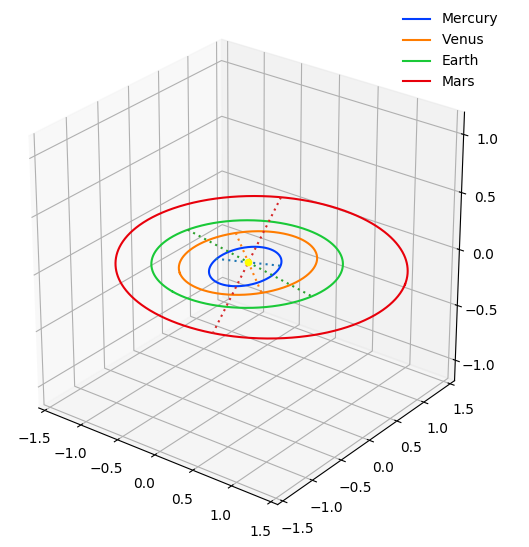
\includegraphics[scale=0.4]{images/plot_example.png}
\caption{Órbitas de Mercurio, Venus, la Tierra y Marte dibujadas con el método \texttt{plotOrbit}.}
\label{fig:plot_example}
\end{figure}


Dado que ya tenemos una estructura para almacenar las coordenadas astronómicas de un objeto y un método que es capaz de representar la elipse definida por dichos elementos, es momento de ponernos a trabajar en la función que nos calcule los elementos orbitales a partir de la posición y velocidad. El código encargado de esta funcionalidad se encontrará en \texttt{scripts/orbital\_elements.py}, y simplemente seguirá los pasos descritos en \ref{sec:elements_determination} para realizar todos los cálculos a partir de la posición y velocidad pasadas como parámetros. Tras hacer los cálculos pertinentes, devolverá un objeto de la clase \texttt{OrbitalObject} con todos los valores obtenidos y como nombre el que se le haya pasado a la función.\\

Así, ya podemos hacer distintas comprobaciones del funcionamiento del código. Nos basta con ir a la efemérides de JPL \cite{jpl}, seleccionar el cuerpo que queramos y anotar su posición y velocidad en un instante $t$. A continuación, utilizamos la función \texttt{getOrbitalElements} pasándole los valores escogidos anteriormente, y podremos dibujar la órbita del objeto que nos devuelva con el método \texttt{plotOrbit}. Un ejemplo de este proceso lo podemos ver en el archivo \texttt{test/test\_1.py}.\\

Una vez explicado el funcionamiento para la representación de datos, pasemos a la parte importante del trabajo, el método de Laplace.\\

\subsection{Implementación del método de Laplace.}
\label{subsec:laplace_method_code}
El desarrollo informático del método de Laplace está basado en una función a la que, pasada una serie de parámetros que contendrán las observaciones de un cuerpo, llamará a una serie de sub-funciones, cada una correspondiente a uno de los pasos vistos en \ref{chap:laplace_method}, y devolverá la posición y velocidad de ese cuerpo en el momento correspondiendo a la segunda observación. Podemos entenderlo mejor con el siguiente pseudocódigo.
\begin{lstlisting}[style=PythonCode]
def Laplace(coordinates, times):
   # Pasamos de ascension recta y declinacion a cartesianas
   position = toCartesian(toRadian(coordinates))
   # Transformamos a dias Julianos
   times = toJulian(times)
   # Calculamos las derivadas (aproximadas)
   EC,EC`,EC`` = approximateDeriv(coordinates,times)
   # Tomamos de la web de JPL el vector Tierra-Sol
   SE,SE`,SE``,R = vectorSE(times[1])
   # Calculamos las distancias $\rho$ y $r$
   rho, r = get_rho_r(EC,EC`,EC``,SE,R)
   # Obtenemos los vectores de posicion y velocidad
   pos, vel = getPosVel(EC,EC`,EC``,SE,SE`,R,r,rho)
   
   Devuelve pos, vel
\end{lstlisting}

Para empezar, tomaremos los valores que se han pasado por parámetro, los cuáles están en ascensión recta y declinación y en formato fecha y hora (año-mes-día hora:minuto), y los pasamos a ecuaciones cartesianas mediante \eqref{eq:equatorial_to_cartesian} y a días julianos \cite{julian}, respectivamente.\\

Continuamos con la función \texttt{approximateDeriv}, que hará exactamente lo que dice su nombre. Utilizando interpolación de Lagrange, se aproximará la primera y segunda derivada del vector $\overrightarrow{EC}$, como hicimos en \ref{sec:series_potencias}.\\

Antes de continuar con el funcionamiento de estas funciones, recordemos las ecuaciones \eqref{eq:relacion_C_S_E}:
\[
\left\{
\begin{array}{l}
	x=\rho\lambda-X\\
	y=\rho\mu-Y\\
	z=\rho\nu-Z
\end{array}
\right.
\]

Tal y como vimos, estas ecuaciones representaban las relaciones entre los tres cuerpos que nos interesan, $C$, $E$ y $S$. Pero para poder resolverlas necesitamos conocer el valor del vector $(X,Y,Z)$. Dado que sería muy cansado tener que tomar la posición (y la velocidad) del Sol de la efemérides cada vez que quisiéramos hacer una aproximación, nos encargaremos de que nuestro programa pueda tomar ese valor automáticamente. Y aquí surge otro problema: no podemos almacenar junto al programa la posición del Sol respecto a la Tierra en todo momento, pues aumentaría el tamaño de este considerablemente. De ahí surge la necesidad de realizar web scraping.\\

\subsubsection{Web Scraping}
La técnica de web scraping es un proceso mediante el cuál podemos obtener información de Internet de manera automatizada. Es una herramienta potente con la que incluso podemos rellenar formularios de manera automática y obtener en formato HTML la página resultante \cite{webscraping}. Para nuestro caso no tendremos que profundizar tanto en las funcionalidades del web scraping, ya que la web de JPL \cite{jpl} nos facilita la obtención de la información del cuerpo que queramos a partir de la URL.\\

De esta manera, definimos en \texttt{util/utilities.py} una función llamada \texttt{getVectorsFromEphemeris} que reutilizaremos a lo largo de la implementación. A dicho método le pasaremos como parámetros los nombres de los cuerpos que $A$ y $B$ que formarán el vector $\overrightarrow{AB}$, el momento en el que queremos tomar el valor del vector y el plano de referencia utilizado (ICRF o eclíptica). Con estos valores formará una \texttt{string} que se corresponderá con la URL que nos devolverá la información requerida. Tras ello, con los paquetes \textit{requests} y \textit{csv} extraeremos la información de la web con dicha URL, a la vez que gestionamos los distintos errores que pueden ocurrir. Finalmente, si todo ha salido bien, se devolverán los vectores de posición y velocidad requeridos y una variable \texttt{True}, y si ha habido algún error, se devolverán vectores de ceros y una variable \texttt{False}.\\

Utilizaremos esta función al llamar al método \texttt{vectorSE}, obteniendo la posición y velocidad del Sol visto desde la Tierra utilizando el plano de referencia ICRF. También se obtendrá el valor de la segunda derivada mediante \eqref{eq:ley_gravitacion_S_E} y la distancia Tierra-Sol, devolviendo finalmente estos cuatro elementos.\\

\subsubsection{Determinación de $\rho$ y $r$ : método de Newton.}
El código desarrollado para determinar $r$ y $\rho$ es el más complejo. Para el cálculo de estos dos valores utilizaremos las secciones \ref{sec:distancias_r_rho} y \ref{sec:newton_rhapson}.\\

La función consistirá en ir calculando los valores de $D$, $D_1$, $N$ y $\psi$ para así llegar a las cantidades $m$ y $M$ de la ecuación \eqref{eq:phi_solution}:
\[
\sin^4{\phi}=M\sin{(\phi+m)}
\]

Una vez tengamos estos valores, iremos utilizando el método de separación de raíces en $[0,\pi]$ para encontrar los subintervalos con una raíz en ellos, y aplicando en su valor intermedio el método de Newton, tal y como vimos en \ref{sec:newton_rhapson}, podremos obtener todas las raíces.
\begin{lstlisting}[style=PythonCode]
def approximate_phi(M,m,tol=1E-09,max_tries=64,plot=False):	
   f = sin(x)^4 - M * sin(x+m)
   
   # Aplicamos el metodo de separacion de raices de Bolzano
   Desde i = 0 hasta max_tries:
      alpha_i = (i*pi) / max_tries
      alpha_{i+1} = ((i+1) * pi) / max_tries
      
      # Si encontramos una raiz en el intervalo ...
      Si signo(f(alpha_i)) != signo(f(alpha_{i+1})):
         # ... tomamos el valor intermedio ...
         x_0 = (alpha_i + alpha_{i+1}) / 2
         
         # ... aplicamos el metodo de Newton ...
         phi, n_iters = newton(f, x_0, tol)
         
         # ... y anyadimos la raiz al resto
         phi_values.anyade(phi)
   
   Si plot:
      dibuja(sin(x)^4)
      dibuja(M * sin(x+m))
      dibuja(phi_values)
   
   Devuelve phi_values
\end{lstlisting}

Además, podremos mostrar si queremos una gráfica por pantalla de la intersección de las funciones junto a las raíces aproximadas, como vemos en el siguiente ejemplo:

\begin{figure}[H]
\centering
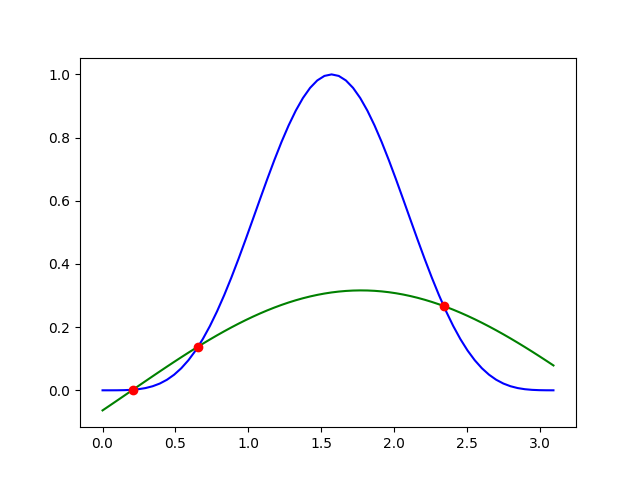
\includegraphics[scale=0.6]{images/example_newton.png}
\caption{Ejemplo de la gráfica que muestra la función \texttt{approximate\_phi} junto a los valores de $\phi$ aproximados.}
\end{figure}

Tras obtener todos los posibles valores de $\phi$ en el intervalo $[0,\pi]$, comprobaremos cuál de ellos es igual a $\pi-\psi$ para discernir entre cuál de los dos restantes es la solución del problema físico, como hicimos en la parte final de \ref{sec:distancias_r_rho}. En el caso de que la solución sea única, se devolverá el valor dicho valor, y si la solución es doble se avisará de ello por pantalla, dando la opción al usuario de elegir entre uno de los dos valores como solución del problema. Se deja para una futura implementación la posibilidad de añadir una cuarta observación para determinar en el caso de una solución doble cuál de las dos es la correcta.\\

Finalmente, con este valor de $\phi$ calcularemos las distancias $r$ y $\rho$ usando \eqref{eq:triangle_relations_2}, y devolveremos estos valores.\\

\subsubsection{Posición y velocidad del cuerpo.}
Una vez hemos obtenido los vectores $\overrightarrow{EC}$ y $\overrightarrow{SE}$ y sus derivadas junto a las distancias $R$, $r$ y $\rho$, solo tendremos que utilizar \eqref{eq:relacion_C_S_E} y \eqref{eq:relacion_C_S_E_derivada} para obtener la posición y velocidad del cuerpo observado.\\

Nótese que los valores obtenidos están respecto al plano ICRF, por lo que una vez que hayamos aplicado por completo el método de Laplace, usaremos la función \texttt{ICRS\_to\_ecliptic} para pasarlos al plano de la eclíptica, tal y como se ha visto en \ref{sec:reference_plane}.\\

\subsection{Estudio del error.}
Para obtener una estimación de cómo de buena ha sido la aproximación del objeto mediante el método de Laplace, se implementarán una serie de funciones para estudiar la diferencia de estas aproximaciones con el valor real.\\

El método \texttt{getApproximationError} tomará como parámetros la posición y velocidad aproximada mediante el método laplaciano de un cuerpo en un instante $t$, así como el nombre del cuerpo que se ha decidido aproximar. Mediante dicho nombre, llamaremos a la función \texttt{getVectorsFromEphemeris} comentada anteriormente para obtener el valor real de la posición y velocidad del cuerpo en el instante $t$ pasado como parámetro. Obtenidos los valores reales, bastará con comprobar la diferencia con los valores aproximados y sus normas, que la función almacenará en una variable \texttt{string}\footnote{Se ha escogido una variable del tipo \texttt{string} para facilitar la impresión por pantalla para la interfaz gráfica.} y devolverá al terminar.\\

\section{Desarrollo de una interfaz gráfica de usuario.}
Todo el código descrito anteriormente es completamente funcional, pero su uso a través de los ficheros en \texttt{tests/} es complicado y poco elegante. Es por ello que nos disponemos a realizar una interfaz gráfica para que la aplicación sea accesible a un mayor número de personas.\\

Como se ha comentado anteriormente, para desarrollar la GUI requerida utilizaremos únicamente el paquete \textit{Tkinter} que viene por defecto en la instalación de Python. La interfaz gráfica implementada se compone básicamente de un formulario en el que introducir los valores de las observaciones y el nombre del cuerpo observado, una serie de botones para realizar distintas funciones con dichos valores y una caja de texto donde mostrar los resultados.

\begin{figure}[H]
\centering
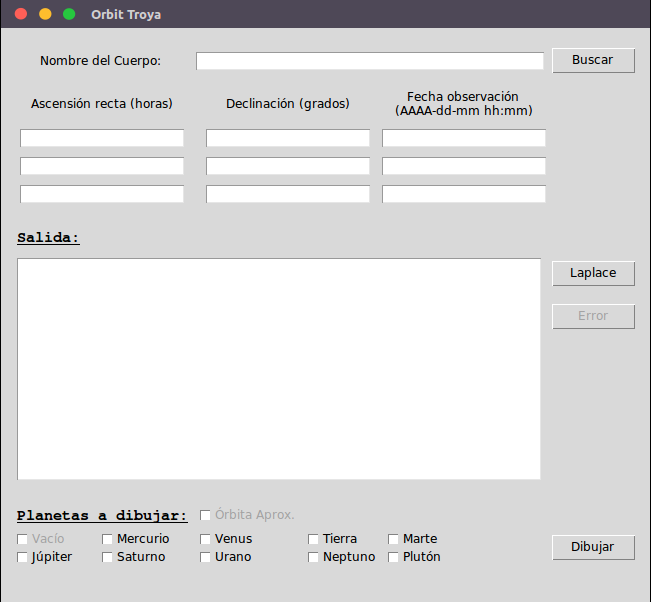
\includegraphics[scale=0.5]{images/gui.png}
\caption{Interfaz gráfica de usuario desarrollada para el método de Laplace.}
\label{fig:gui}
\end{figure}

Para empezar, creamos el directorio \texttt{gui/} que contendrá en su interior un fichero con la definición clase \texttt{OrbitTroya}. En el constructor de esta clase inicializaremos todos los elementos del paquete \textit{Tkinter} que vamos a mostrar en la interfaz y los posicionaremos en el \texttt{grid}.
\begin{itemize}
\item \texttt{Label} para poner los títulos (``Nombre del Cuerpo'', ``Salida:'', etc).
\item \texttt{Entry} para introducir los valores (casillas bajo ascensión recta, declinación y fecha).
\item \texttt{Text} para mostrar los resultados (bajo ``Salida'').
\item \texttt{Checkbutton} para elegir entre los distintos planetas a dibujar (Mercurio, Venus, Tierra, etc).
\item \texttt{Button} para realizar distintas funcionalidades (Buscar, Laplace, Error, Dibujar).
\end{itemize}

Los elementos realmente interesantes para explicar su implementación son los \texttt{Button}, los cuáles contendrán un atributo \texttt{command} y al pulsar sobre ellos llamarán a la función de dicho atributo. Veamos su funcionamiento uno a uno.\\

El botón ``Buscar'' se encargará de tomar el nombre introducido a su izquierda\footnote{Para que funcione correctamente, el nombre debe de ser el oficial proporcionado por el JPL.} y buscar en la efemérides su posición y velocidad respecto al Sol con la función \texttt{getVectorsFromEphemeris} comentada anteriormente. Además, con estos valores calculará las coordenadas astronómicas del objeto buscado. En caso de que se encuentre en la efemérides, se mostrará un mensaje de éxito en el cuadro de texto y se dará la opción de dibujar la órbita de dicho objeto, poniendo el nombre del cuerpo en el \texttt{Checkbutton} ``Vacío'' de la imagen \ref{fig:gui} y haciendo éste botón seleccionable. En caso contrario, se mostrará un mensaje de error en el cuadro de texto y el \texttt{Checkbutton} seguirá igual. Esta funcionalidad está realmente pensada para comparar la órbita real y la aproximada del objeto una vez hayamos aplicado el método de Laplace.\\

Si pulsamos en el botón ``Laplace'', el programa tomará los valores introducidos en el formulario y llamará al método \texttt{Laplace} que vimos en \ref{subsec:laplace_method_code}. Tras ello, pasará las coordenadas de ICRF a la eclíptica, calculará las coordenadas astronómicas, mostrará toda esta información en el cuadro de texto y dará la opción de pinchar en el bóton ``Error''. Finalmente, comprobará si la órbita se puede dibujar (es decir, que $a>0$) y si es así hará seleccionable el \texttt{Checkbutton} ``Órbita Aprox.''.\\

Respecto al botón ``Error'', simplemente tomará los valores de la posición y velocidad aproximados mediante Laplace y mostrará por pantalla el resultado del método \texttt{getApproximationError}.\\

Finalmente, el botón ``Dibujar'' se ocupará de comprobar cuáles de los \texttt{Checkbutton} de su izquierda están seleccionados, añadiéndolos a una lista y llamando al método \texttt{plotOrbit}. Los valores para dibujar los planetas del Sistema Solar estarán almacenados en \texttt{utils/my\_constants.py}.\\

Aunque este programa esté hecho para aplicar el método de Laplace, es curioso que sin darnos cuenta hemos desarrollado un programa capaz de dibujar la órbita de cualquier objeto del Sistema Solar junto a los principales planetas (y Plutón). Bastará con introducir el nombre del cuerpo que queramos dibujar su órbita y darle al botón ``Buscar'', obteniendo de tal manera la posibilidad de dibujar la elipse que forma su movimiento alrededor del Sol.\\


\chapter{Experimentación y resultados}
\label{chap:experimentation}
Una vez que hemos desarrollado un software específico para aproximar la órbita de un objeto mediante el método de Laplace, comprobemos su correcto funcionamiento, así como cómo de buenas son los las aproximaciones obtenidas con el método Laplaciano.\\

Dado que no disponemos de instrumental óptimo para realizar las observaciones por nuestra cuenta, utilizaremos (una vez más) la efemérides online del JPL \cite{jpl}, con la que podemos obtener la ascensión recta y declinación observada desde la Tierra de cualquier objeto en cualquier momento. De esta manera, comencemos a ver diferentes resultados prácticos y comentemos la eficacia del método de Laplace que hemos estudiado.\\

\section{Cuando el cuerpo es cercano: Ceres.}
\label{sec:exp_ceres}
Tal y como hemos contado en \label{sec:history}, en 1801 Giuseppe Piazzi descubría el planeta enano Ceres, y meses más tarde Gauss usaba su recientemente desarrollado método para obtener la órbita del objeto con las observaciones que Piazzi había anotado. Gracias a ello, pudieron recuperar la pista de este planeta enano.\\

En ese momento quedó demostrado que el método de Gauss hacía buenas estimaciones para cuerpos a una distancia aproximada a la de Ceres. ¿Hubiera conseguido Laplace unos resultados exitosos? Veámoslo.\\

Vamos a tomar la ascensión recta y declinación de Ceres para ciertos momentos entre los días 28 y 30 de julio de 2020. Los introducimos en el programa desarrollado junto a su nombre, quedando de la siguiente manera:
\begin{figure}[H]
\centering
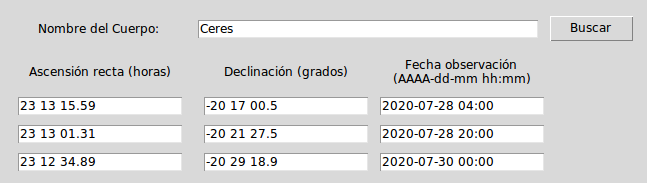
\includegraphics[scale=0.5]{images/ceres_exp.png}
\caption{Datos de Ceres introducidos en el programa.}
\label{fig:ceres_exp}
\end{figure}

Cuando pulsemos el botón ``Buscar'' encontrará en la efemérides el cuerpo requerido de manera satisfactoria.
\begin{lstlisting}[style=Console]
Órbita de Ceres obtenida.
Ahora puedes dibujar el objeto junto al resto.

Nombre = 'Ceres'
a = 2.7672121143653663 UA
e = 0.07772816968324102
i = 10.588147218912999 grados
(*$\Omega$*) = 80.28170111757919 grados
(*$\omega$*) = 73.71539237319364 grados
Período = 1681.3979070284568 días
\end{lstlisting}

A continuación, veamos qué tal funciona el método de Laplace. Con dichos valores, obtenemos los siguientes posibles valores para $\phi$:
\[
\left\{
\begin{array}{l}
\phi_1=11.9311189º\\
\phi_2=37.60583084º\\
\phi_3=134.04867322º
\end{array}
\right.
\]

Dado que $\psi=142.39416916267487º$, cuando calculemos $\pi-\psi$ veremos que es igual a $\phi_2$, por lo que la solución será única y se corresponderá con $\phi_1$.\\

En vez de mostrar el resultado de aplicar el método laplaciano y calcular los elementos orbitales (será más visual compararlo en una gráfica), veamos directamente el error con su valor real utilizando el botón ``Error'':
\begin{lstlisting}[style=Console]
Posición real: [ 2.53436621 -1.48439324 -0.51379219]
Posición calculada: [ 2.54870673 -1.48940124 -0.51764288]
Error = [-0.01434052  0.005008    0.00385069]
|Error| = 0.01567030503509054

Velocidad real: [ 0.00478149  0.00826443 -0.0006202 ]
Velocidad calculada: [ 0.00496131  0.00816816 -0.00068937]
Error = [-1.79816103e-04  9.62781299e-05  6.91715556e-05]
|Error| = 0.0002153787671514888

Distancia real: 2.9816803651312407
Distancia aproximada: 2.9970278967029773
\end{lstlisting}

Podemos observar que la aproximación en $t=$2020-07-28 20:00 es muy buena a pesar de que se haya realizado con tan solo tres observaciones del cuerpo desde la Tierra. Aún así, hay que tener en cuenta que un error en la distancia de $0.01$ UA se corresponde con $1495978.707$ kilómetros.\\

Para terminar, utilicemos las coordenadas astronómicas que hemos aproximado de Ceres para dibujar la órbita asociada a estas coordenadas. Además, añadiremos la órbita real para comprobar cómo de buena es la aproximación, y la órbita de la Tierra para hacernos una pequeña idea de la distancia del cuerpo que hemos utilizado.

\begin{figure}[H]
\centering
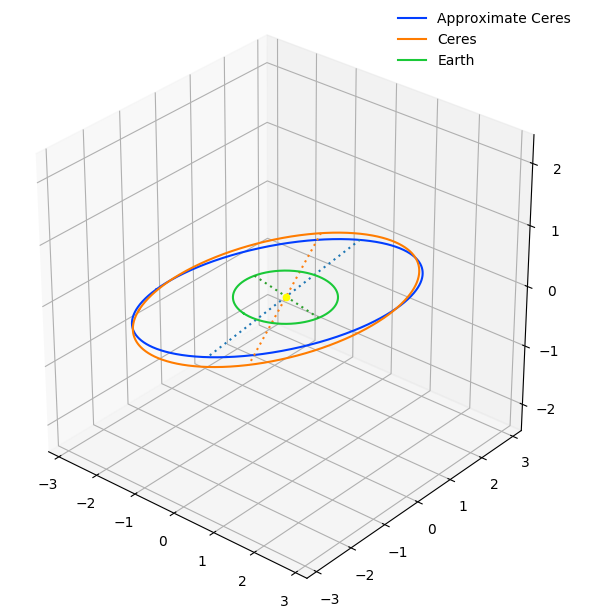
\includegraphics[scale=0.4]{images/plot_ceres.png}
\caption{Órbita real y aproximada de Ceres junto a la Tierra.}
\label{fig:plot_ceres}
\end{figure}

Es fácilmente observable que los elementos orbitales obtenidos a través de la aproximación son muy similares a los reales, y con dicha órbita aproximada podríamos encontrar el planeta enano Ceres en la bóveda celeste. Por tanto, el método de Laplace hubiera sido tan válido como el de Gauss para que en 1801 se hubiese recuperado el cuerpo en el cielo nocturno.\\

\section{El error aumenta con la distancia: Hilda y Plutón.}
\label{sec:exp_hilda_pluton}
Ya hemos visto que con un cuerpo relativamente cercano funciona bien el método de Laplace. Alejémonos un poco más.\\

Empecemos tomando el asteroide Hilda (A875 VC en la efemérides), un objeto que da nombre a un grupo de asteroides situado a unas cuatro unidades astronómicas, entre la órbita de Júpiter y el cinturón de asteroides. Tomamos su ascensión recta y declinación de la efemérides, las introducimos en el programa y aplicamos el método de Laplace.\\

\begin{figure}[H]
\centering
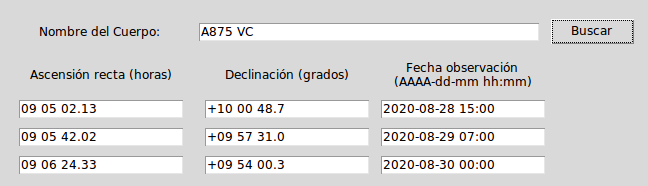
\includegraphics[scale=0.5]{images/hilda_exp.png}
\caption{Datos de Hilda (A875 VC) introducidos en el programa.}
\label{fig:hilda_exp}
\end{figure}

Antes de dar un resultado para la posición y velocidad del cuerpo, el programa para, ya que ha encontrado una solución doble, y nos preguntará sobre cuál de los dos valores posibles queremos tomar como solución del problema físico.\\
\[
\left\{
\begin{array}{l}
\phi_1=4.35491299º\\
\phi_2=18.19187998º\\
\phi_3=158.82202981º=\pi-\psi
\end{array}
\right.
\]

Si escogiésemos $\phi_2$ estaríamos tomando un ángulo mayor al que se encontró como solución en el caso de Ceres, lo cuál no tendría sentido, pues a mayor distancia del cuerpo, menor ángulo forma con la Tierra y el Sol; por tanto, elegiremos como solución $\phi_1$. Nótese que este razonamiento no se podría haber hecho en un caso real de determinación de órbitas, pues a priori no sabemos si el objeto está mas cerca o más lejos con una simple observación.\\

Veamos el resultado que se obtiene tras discernir entre cuál de las dos soluciones es la buena:
\begin{lstlisting}[style=Console]
Aproximación en t = 2020-08-29 07:00:00.000
Posición calculada: [-3.16680643  3.55611002 -0.63839816]
Velocidad calculada: [-6.72694445e-03 -7.39134996e-03 -6.61539321e-05]

Elementos orbitales obtenidos:
Nombre = 'Approximate A875 VC'
a = 12.704405560669025 UA
e = 0.6270295383846635
i = 7.72591356505979 grados
(*$\Omega$*) = 129.50904027965768 grados
(*$\omega$*) = 276.6199742996565 grados
Período = 16540.108377222892 días
\end{lstlisting}

\begin{lstlisting}[style=Console]
Posición real: [-2.83281544  3.23203176 -0.58633104]
Posición calculada: [-3.16680643  3.55611002 -0.63839816]
Error = [ 0.33399099 -0.32407826  0.05206712]
|Error| = 0.46828163075398077

Velocidad real: [-5.32298460e-03 -5.80807100e-03 -1.18918535e-05]
Velocidad calculada: [-6.72694445e-03 -7.39134996e-03 -6.61539321e-05]
Error = [1.40395985e-03 1.58327896e-03 5.42620785e-05]
|Error| = 0.002116794723497365

Distancia real: 4.337586507139335
Distancia aproximada: 4.804386918636096
\end{lstlisting}

Aunque el error en la aproximación de la posición y la velocidad no es excesivamente grande, parece que la cosa no ha ido demasiado bien a la hora de pasar a coordenadas astronómicas, pues habíamos comentado previamente que la distancia del asteroide al Sol era aproximadamente 4 UA, mientras que hemos obtenido una distancia de 12 UA. Veamos una imagen de la órbita calculada junto a la real y las órbitas de la Tierra y Júpiter.

\begin{figure}[H]
\centering
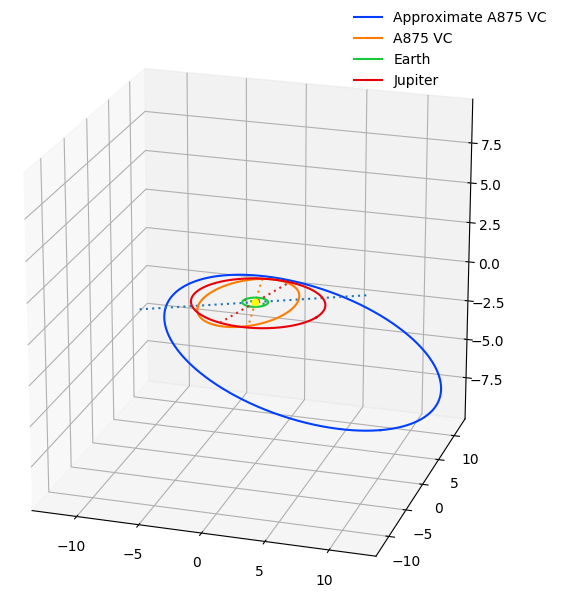
\includegraphics[scale=0.5]{images/hilda_plot.png}
\caption{Órbita real y aproximada de Hilda (A875 VC) junto a la Tierra y Júpiter.}
\label{fig:hilda_plot}
\end{figure}

La aproximación ha sido bastante mala, por lo que no sería mala idea probar con otras observaciones, teniendo en cuenta que podríamos tomarlas más o menos espaciadas que en el caso que hemos estudiado.\\

Comprobemos rápidamente si alejándonos más todavía del Sol sigue aumentando el error de aproximación. Vayámonos muy lejos, concretamente a Plutón. Tomemos sus coordenadas ecuatoriales en tres momentos diferentes y veamos qué tal se porta el método de Laplace.\\

El método se aplica y obtiene una solución de $\phi$ única; en vez de mostrar todo el error, veamos solamente qué tal ha aproximado la distancia al planeta en $t=$2020-09-14 19:00.

\begin{lstlisting}[style=Console]
Posición real: [ 13.74165616 -31.22436196  -0.6327821 ]
Posición calculada: [  7.74035668 -16.5876921   -0.33519062]
Error = [  6.00129948 -14.63666986  -0.29759148]
|Error| = 15.822018227154214
\end{lstlisting}

Con esto podemos ir empezando a sospechar que cuanto mayor sea la distancia al cuerpo observado, mayor será el error que acarrea la aproximación de su posición y velocidad. Es más, el error en esta aproximación hará que al calcular los elementos orbitales obtengamos un semieje mayor negativo, algo que no es posible, y esta aproximación debería ser descartada como solución del problema físico.

\begin{lstlisting}[style=Console]
Aproximación en [...]

Elementos orbitales obtenidos:
Nombre = 'Approximate 999'
a = -0.0019409803348728837 UA
e = 581.0174156903244
[...]

Semieje mayor negativo, no se puede dibujar la órbita.
\end{lstlisting}

\vspace{0.5cm}

\section{Cuerpos muy excéntricas: C/2020 F3 (Neowise).}
\label{sec:neowise}
Cuanto mayor sea la excentricidad de un cuerpo espacial, más alejado estarán sus focos, pero más se acercará a ellos en algún momento de su órbita. Este es el caso del objeto C/2020 F3 (Neowise), un cometa del que se oyó mucho hablar durante el pasado mes de julio debido a que, en su trayectoria alrededor del Sol, se acercaba al punto más cercano a la Tierra, de manera que se podía observar a simple vista, y no volvería a ser así hasta dentro de 6765 años.\\

Hemos visto que con objetos muy lejanos la aproximación que nos da el método de Laplace es muy mala. Pero, ¿y si las medidas se toman cuándo el objeto esté muy cercano a la Tierra, de manera que las observaciones sean incluso mejores que las de Ceres?\\

Escogemos los valores de las observaciones del cometa entre el día 14 y el día 15 de julio, en los que su posición en la órbita se encontraba muy cerca de la Tierra.
\begin{figure}[H]
\centering
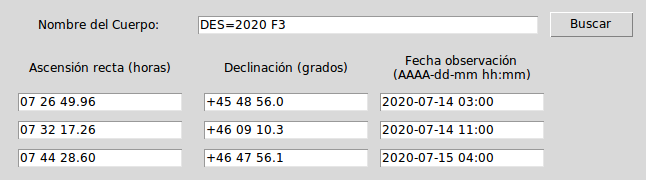
\includegraphics[scale=0.5]{images/neowise_exp.png}
\caption{Datos de C/2020 F3 (Neowise) introducidos en el programa.}
\label{fig:neowise_exp}
\end{figure}

Al aplicar el método de Laplace, volvemos a obtener una solución doble, $\phi_1=90.35678364º$ y $\phi_2=107.33111728º$. En este caso no podemos decidir fácilmente entre cuál de las dos es la válida por lo que elegimos, por ejemplo, $\phi_2$ (y tendremos suerte con la elección). Tras la ejecución, comprobamos el error con la posición y velocidad real en el instante que hemos aproximado.
\begin{lstlisting}[style=Console]
Posición real: [ 0.16652972 -0.24402154  0.32665628]
Posición calculada: [ 0.16854806 -0.25029356  0.32362519]
Error = [-0.00201834  0.00627202  0.00303109]
|Error| = 0.0072525445535108184

Velocidad real: [-0.01084886 -0.03392851  0.00860642]
Velocidad calculada: [-0.0106734  -0.03331783  0.00864502]
Error = [-1.75460689e-04 -6.10680287e-04 -3.85976705e-05]
|Error| = 0.0006365584389714605

Distancia real: 0.44043499684292076
Distancia aproximada: 0.4424800312802405
\end{lstlisting}

Como vemos, los errores al calcular los vectores de posición y velocidad son muy pequeños, hecho que era de esperar al estar tan cerca el objeto que se ha observado. ¿Tendremos la misma suerte con el cálculo de los elementos orbitales?,\\

Comencemos viendo qué tal ha ido la aproximación para la excentricidad y los ángulos $i$, $\Omega$ y $\omega$, comparando los valores en la siguiente tabla.
\begin{table}[H]
\centering
\resizebox{8cm}{!}{%
\begin{tabular}{ccc}
         & \textit{Valor real}         & \textit{Valor aproximado}   \\ \hline
$e$      & $0.9992401080381621$ & $0.9623385094824053$ \\ \hline
$i$      & $128.9372837890982$  & $129.87582386324678$ \\ \hline
$\Omega$ & $61.01063124644879$  & $60.32375719162504$  \\ \hline
$\omega$ & $37.28105014282296$  & $34.302810750239566$
\end{tabular}%
}
\end{table}

Parece que todo ha ido bien, por lo que veamos ahora una imagen comparando las dos órbitas.

\begin{figure}[H]
\centering
\subfloat{
	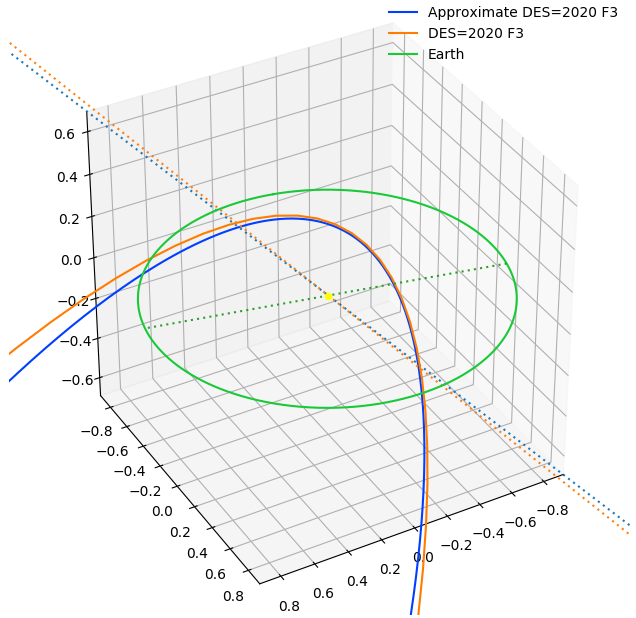
\includegraphics[scale=0.275]{images/neowise_close.png}
	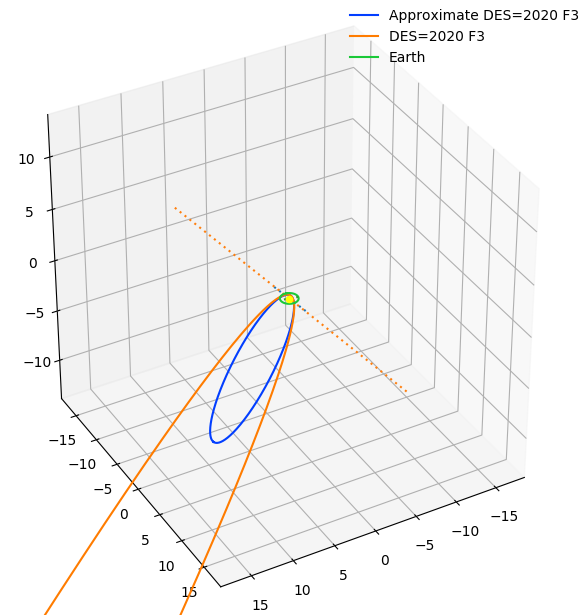
\includegraphics[scale=0.275]{images/neowise_far.png}
}
\caption{Órbita real y aproximada de C/2020 F3 (Neowise) junto a la Tierra vista desde cerca y desde lejos.}
\label{fig:neowise_plot}
\end{figure}

En este caso, observando la órbita de cerca, tenemos una muy buen aproximación, pero conforme nos vamos alejando nos damos cuenta de que ha habido un error muy grande en el semieje mayor: el valor aproximado de $a$ es 7.640204712942875 UA, mientras que el real es de 387.7566248050956 UA, 380 UA de diferencia.\\

Para entender el por qué de este error tan grande tenemos que volver a la sección \ref{sec:elements_determination} y recordar el cálculo de $a$:
\[
h=\frac{|v(t)|^2}{2}-\frac{\mu}{|r(t)|}
\]
\[
a=-\frac{\mu}{2h}
\]

Por tanto, el valor de $a$ depende únicamente del valor de la energía, que se calcula a partir de la norma de la posición y la velocidad. Si tomamos el valor de $a$ como una función en $h$, estaremos ante una función hiperbólica, la cuál diverge cuando se acerca a 0. Para que el valor de $a$ sea muy grande, la energía debe de ser muy cercana a 0, de manera que, por el hecho de que $a$ diverge en 0, el mínimo error en la energía puede causar un error muy grande en el cálculo del semieje mayor, y esto es lo que ha ocurrido en el caso de C/2020 F3 (Neowise).










\newpage

\begin{thebibliography}{99}

\bibitem{numpy} \textsc{Oliphant, T.E. et al.}, (2020), Numpy (1.18.5) and Scipy (1.4.1) [library documentation]. Obtenido de \href{https://docs.scipy.org/doc/}{link}.

\bibitem{matplotlib} \textsc{Hunter, J.D. \& Droettboom, M}, (2020), Matplotlib (3.0.3) [library documentation]. Obtenido de \href{https://matplotlib.org/3.0.3/index.html}{link}.

\bibitem{seaborn} \textsc{Waskom, M.}, (2020), Seaborn (0.9.1) Color Palette [library documentation]. Obtenido de \href{https://seaborn.pydata.org/tutorial/color_palettes.html}{link}.

\bibitem{astropy} \textsc{The Astropy Developers}, (2020) Astropy (3.2.3) [library documentation]. Obtenido de \href{https://docs.astropy.org/en/stable/index.html}{link}.

\bibitem{requests} \textsc{Reitz, K.}, (2020), Requests (2.9.1) [library documentation]. Obtenido de \href{https://requests.readthedocs.io/_/downloads/es/es/latest/pdf/}{link}.

\bibitem{sympy} \textsc{SymPy development team}, (2020), Sympy (1.6.2) [library documentation]. Obtenido de \href{https://docs.sympy.org/latest/index.html}{link}.

\bibitem{tkinter} \textsc{Lundh, F.}, (2020), Tkinter (3.5.1-1) [library documentation]. Obtenido de \href{https://docs.python.org/3/library/tk.html}{link}.

%\bibitem{webscraping} \textsc{Alonso Burgos, S.}, (2020), \textit{"Teoría" de Web Scraping} [Archivo de vídeo]. Recuperado de [vídeo oculto].

\bibitem{webscraping} \textsc{Breuss, M.}, (2019), Beautiful Soup: Build a Web Scraper With Python. Lugar de publicación: \textit{Real Python}, \href{https://realpython.com/beautiful-soup-web-scraper-python/}{link}.

\bibitem{julian} \textsc{Cirillo, J.}, (2015), Día Juliano. Lugar de publicación: \textit{El manual de KStars}, \href{https://docs.kde.org/trunk5/es/extragear-edu/kstars/ai-julianday.html#:~:text=El%20n%C3%BAmero%20de%20d%C3%ADas%20se,n%C3%BAmeros%20de%20sus%20d%C3%ADas%20julianos.}{link}



\end{thebibliography}

\end{document}

